\chapter{相关工作}
\label{chap:intro}

为了保证软件的可靠性和稳定性,在大量研究人员长期不懈地努力下,出现了很多针对软件缺陷的检测方法。这些方法可以在软件开发周期的不同阶段介入,检测的效率和效果也大不相同,最终涌现出了一批相对成熟的代码缺陷检测方法和工具。另一方面,随着软件数量的日益庞大,以及数据挖掘技术在各个研究领域的广泛应用,利用机器学习的方式来解决软件安全问题也逐渐成为了研究热点。

\section{程序静态分析技术}

静态分析技术即是在不运行程序,不依赖程序输入的情况下对程序代码进行分析的一项技术。这种技术有助于开发人员对代码结构的理解,同时也能检测潜在的安全缺陷(如SQL注入),运行时错误(如空指针引用缺陷)以及部分代码逻辑错误。它一般需要配合利用自动化工具执行分析。采用的技术有数据流分析,机器学习,语义精简等。可检测死锁,空指针,资源泄露,缓存区溢出,安全漏洞,竞态条件等软件缺陷,具有快速,准确,伸缩性强等特点。能够在代码开发阶段找到并修复多种问题,从而节省大量人力成本和时间。下面对部分静态分析方法涉及的相关技术进行简要的介绍。

符号执行\cite{king1976symbolic}是静态分析中较常用到的一种技术,它可以利用抽象符号描述程序执行过程中的变量值。这种方法可以很好地模拟程序的运行过程。相对于传统方法无法确定程序真实执行下各变量值的情况,此方法在对程序进行路径敏感分析时十分有效。不过因为符号执行方法会追踪程序中所有变量的所有取值空间,所以在应用于大规模代码进行分析时,可能会导致分析的可能路径数量迅速增多,因此在应用该方法的时候,往往会采取优化路径数量的方法即选择部分可能性最高的路径进行分析,这样虽然可以避免状态爆炸的产生,但是也难免会导致分析精度的下降。

PREfix\cite{bush2000static}是一种针对C语言的静态分析工具,它采用了符号执行的方法。该工具可以对程序每个可能的执行过程进行抽象建模,静态地模拟程序的多个可能执行路径,同时利用约束求解对程序分析过程中出现的约束集合进行检查。此工具能够做到路径敏感的缺陷检查,但是由于符号执行方法的特性,为了避免状态爆炸的情况出现,它只能选取部分路径进行分析,这就导致了分析精度的不理想。

模型检查\cite{jhala2009software}也是一种常见的静态分析技术,通常的做法是构建有限状态机或者有向图等抽象模型,再对构造出的模型进行遍历来检验待检测系统的部分性质。SLAM\cite{ball2001automatically}是一种具有代表性的基于模型检查的静态分析工具。它可以从待检测代码中抽象出一个布尔程序并加以验证。在得到的错误报告中逐个检查,找出所有误报,进而根据这些误报对抽象的布尔程序进行调优,经过不断迭代,最终可以取得很好的效果。

同样是应用于程序验证的技术,不同于模型检查,定理证明\cite{tiwari2007logical}是基于语义的程序分析方法。但是由于采用了消解原理的定理证明器,而这种方法对整数域和有理数域相关的运算不是很好处理,所以应用在程序分析领域显得不是特别合适。基于这种问题,研究人员通常会选择各种判定过程来确定公式是否是定理。ESC\cite{flanagan2013pldi}就是一个采用了定理证明技术的半自动化工具,它在分析程序的过程中需要外界指定所涉及的类不变量,过程不变量以及循环不变量。

除了上面提到的3种技术,抽象解释\cite{cousot1977abstract}的应用更加广泛,它是数据流分析的理论基础。1977年P.Cousot和R.Cousot
共同提出了抽象解释的理论,应用该理论分析程序时就不需要拘泥于程序最底层的具体细节上可以在更高的角度上去观察和思考。传统解释器可以知道程序中每个变量具体的值从而得到具体值域,而抽象解释不同与传统解释的地方就是可以得到一个更高阶的抽象值域。如果将一个传统解释器迁移到抽象解释器,几乎等同于构造一个函数把具体值域映射到抽象值域。如图\ref{fig:figure2-1}所示,我们可以将无限的整数具体值域抽象成正,负,零三个抽象值域,这个过程只需要实现一个抽象函数$\alpha$即可完成。
 \begin{figure}
	\centering
	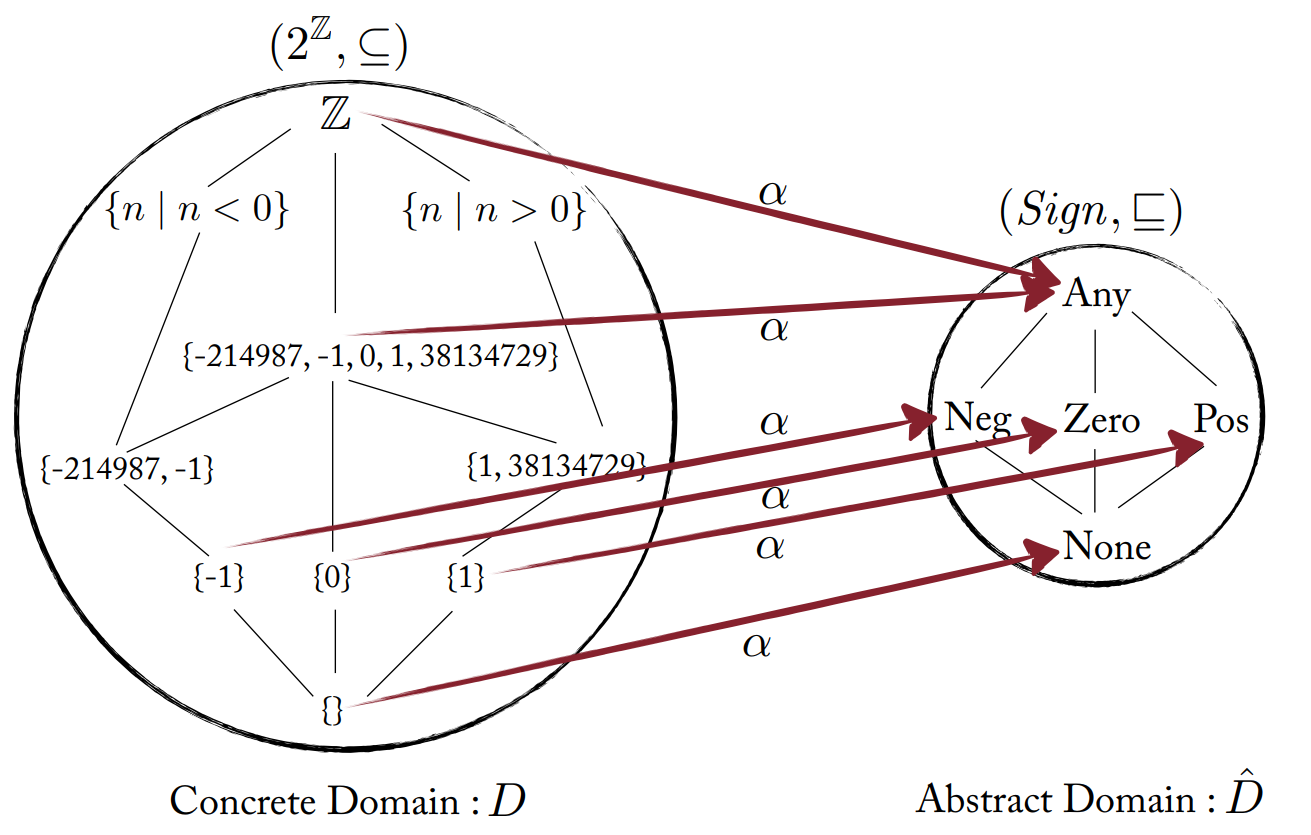
\includegraphics[width=0.70\textwidth]{figures/AbstractInterpretation2-1}
	\caption{将整数空间的具体值域映射到抽象值域}\label{fig:figure2-1}
\end{figure}

抽象解释理论实际上是从代码中抽象出一些能够刻画我们想要分析的问题所需要的特征,本质上还是为了提升分析的效率而损失部分分析精度的方法。但是如果应用得当,还是可以获得很大的收益,现在几乎所有的数据流分析方法都应用了该理论。

总的来说,静态分析技术在不运行代码的情况下进行分析有效避免了程序运行环境的苛刻要求,可以针对程序的规模采取灵活的分析方法,从而具备了较早发现缺陷,较低的分析成本,较高的覆盖率和自动化程序等优点。但是由于往往需要对分析精度进行部分舍弃,导致了分析结果的漏报率和误报率都无法达到特别理想的水平。

\section{静态分析技术在空指针引用缺陷检测的应用}
针对空指针引用缺陷,研究人员已经利用静态分析技术做出了很多实践并取得了一定成果。

研究人员利用静态分析技术在Java空指针引用缺陷上进行了大量的工作,产生了很多检测空指针引用的工具和技术,这些技术可粗略的分为指针引用验证\cite{madhavan2011null}和空指针引用\cite{xie2007saturn}缺陷检测两大类。前者侧重于如何验证程序中的指针是否为空。后者侧重于如何尽可能多的发现程序中的空指针引用。指针引用验证技术是基于需求驱动的思想\cite{wang2015},一般是首先识别出指针,再沿着控制流后向的验证指针是否为空。空指针引用缺陷检测一般是在进行数据流分析\cite{wangxu2015}、指针分析的基础上,根据一些规则基于控制流前向的检测。两者通常都需要进行数据流分析与指针分析。

Salsa\cite{loginov2008verifying}是一个致力于验证Java代码中指针引用安全性验证的工具,通过定制的数据表示形式进行前向数据流分析,通过对传播深度和数据流传播路径数量的简单限制来获得方法的可扩展性,同时依赖预先进行的必然别名分析来提高方法间数据流分析的准确性。由于一些空指针的引用需要经过多层方法调用链才有可能触发,这种验证方式会产生很多漏报的同时,效率也不理想。数据流分析技术具有十分灵活的特点,为了提高效率,Ravichandhran Madhavan\cite{madhavan2011null}等提出了一种过近似的最弱前置条件分析方法以验证Java程序中指针的安全性,该方法通过需求驱动的前向数据流分析大幅提升了单个引用的分析效率,该方法试图找到程序入口处可能满足被分析程序点的引用不安全的条件,如果存在这样的条件,则可以判定该引用不安全。此方法的数据流事实为有限的谓词集合,通过有选择地限制谓词集合的大小以及传播路径的数量,该方法可以做到低延迟的流敏感,上下文敏感的sound分析,利用Wala\cite{wala}程序分析框架,可以取得较好的验证引用安全的效果,但是过于追求针对单个引用的需求驱动分析,在对大规模代码中的引用进行批量分析时性能欠佳。

空指针检测相比于指针安全性验证更加具有实用性,而误报率和漏报率是检验工具实用性的重要指标,空指针检测工具大多不追求完美的正确率,而将较低的误报率和较高的召回率作为最重要的目标。

检测工具Xylem\cite{nanda2009accurate}从每一个指针引用出发,进行基于需求驱动的后向数据流分析,并将谓词作为数据流事实,目标是能够高效的检测出最重要的空指针引用,在进行分析时采取的是不完全可靠的分析方法,检测结果存在较多漏报。

北京邮电大学的杨睿\cite{yangrui2012}提出一种Java中空指针引用故障的静态检测方法,将空指针引用问题抽象为一类故障模型,并以故障模式状态机来形式化描述此类故障模型,然后根据故障状态机的创建条件及待检测代码的语义信息确定是否创建该类型的状态机,并将创建的状态机示例置于控制流图入口,根据数据流分析的结果对故障状态进行迭代以检测空指针引用问题。

中国矿业大学的姜淑娟\cite{jiang2017}提出一种空指针异常自动定位方法,该方法结合程序的静态分析技术,利用程序运行时的堆栈信息指导程序切片,然后对得到的切片进行空指针分析及别名分析,得出引发空指针异常的可疑语句集合,最终给出错误定位报告。

总体来看,以上这些分析方法都有各自的优缺点,但是目前无法找到一种完美的静态检测方法可以兼顾缺陷检测的误报率和漏报率。这也正是静态代码分析的短板,不仅是将复杂的缺陷解释出来很困难,对于结果的高误报率,往往显得无能为力。

\section{代码缺陷检测工具介绍}
对于空指针引用缺陷,工业界已经产生了很多优秀的检测工具,这些工具具有不同的实现原理,对空指针引用缺陷的检测结果也不尽相同。

FindBugs\cite{hovemeyer2005evaluating}\cite{hovemeyer2007finding}是一个开源的针对Java代码的缺陷静态检测工具,通过分析class文件,在字节码层级进行简单的前向数据流分析,对程序中的每一个引用的是否为null值的不同情况,给定相应的标识从而在触发可能的空指针调用时给出不同的告警等级。对于指针引用FindBugs总结出了一些经验规则,对不可达路径、控制流汇合、指针赋值语句、断言等特定情况定制了专用的检测规则,在进行过程间分析时,其主要依赖特定故障模式以及用户编码时给出的注解来推断空指针是否可能发生,所以它只能在特定场景下检测出空指针引用缺陷。

Jlint同样是一个开源静态代码检测工具,它通过执行数据流分析和构建锁图来查找缺陷,语义矛盾和同步问题。Jlint有两个独立的程序来执行语法和语义验证。通过使用手写扫描器和简单的自顶向下解析器,Jlint能够检测到一些代码缺陷,例如可疑地使用操作符优先级,没有切换代码中断,对构造体错误的假设等。同时,Jlint执行本地和全局数据流分析,计算局部变量的可能值并捕获冗余和可疑计算。通过执行全局方法调用分析,Jlint能够检测具有可能为“null”的形参的方法的调用,并且在没有验证“null”的方法中使用该参数。 Jlint还为类依赖项构建了锁依赖关系图,并使用该图来检测在多线程程序执行期间可能导致死锁的情况。除了死锁之外,当不同的线程可以同时访问相同的变量时,Jlint能够检测到可能的竞争条件问题。Jlint最大的特点就是检测的效率很高,但是由于使用的数据流分析十分有限,因此误报率也较高。

Infer是Facebook的开发团队在代码提交内部评审时,用来执行增量分析的一款静态分析工具,在代码提交到代码库或者部署到用户的设备之前找出缺陷。由OCaml语言编写的Infer目前能检测出空指针访问、资源泄露以及内存泄露,可对C、Java或Objective-C代码进行检测。Facebook使用Infer自动验证iOS和安卓上的移动应用的代码,bug报告的正确率达80\%。Infer通过捕获编译命令,把要被编译的文件转换为可用于分析潜在错误的中间语言格式。整个过程是增量进行的,意味着通常只有那些有修改过并提交编译的文件才会被Infer分析。Infer还集成了大量的构建或编译工具,包括Gradle、Maven、Buck、Xcodebuild、clang、make和javac。此外,Infer根植于两大基本理论之上,其一是霍尔逻辑,一种用于推理计算机程序正确性的形式系统,另一个是抽象解释,该理论用于测度程序语义的逼近结果,此外还涉及其它一些研究成果,例如Separation Logic和Bi-abduction。

Fortify SCA是一款应用广泛的商业工具,由知名的惠普公司出品 ,是一个白盒的、静态的软件源代码安全检测工具。它通过内部的五种主要分析引擎:语义、结构、控制流、数据流、配置流等对应用程序的源码进行静态分析,在分析的同时与该工具特有的软件安全漏洞规则集进行全面地查找、匹配,进而找出源代码中存在的各种缺陷和漏洞,并整理和产出缺陷报告。Fortify应用十分广泛,在世界范围内被大量公司用作内部源代码的质量安全检测工具。

Coverity是美国Coverity公司提供的可配置的用于检测软件缺陷和安全隐患的静态源代码分析解决方案,该工具基于布尔可满足验证技术应用于源代码分析引擎,分析引擎利用其专利的软件DNA图谱技术和meta-compilation技术,综合分析源代码、编译构建系统和操作系统等可能使软件产生的缺陷。Coverity是第一个能够快速、准确分析当今的大规模、高复杂度代码的工具,它解决了影响源代码分析有效性的很多关键问题,如编译兼容性,构建集成,高误报率,有效的错误根源分析等。

\section{深度学习技术在软件安全领域的应用}
深度学习是人工神经网络中一种多层级学习框架,试图通过构建深层网络模拟人脑感知抽象概念的能力。近年来,深度学习凭借着强大的特征学习能力,问题表达能力,数据容纳能力,掀起了又一次机器学习的浪潮,并在计算机视觉,语音处理,自然语言处理等众多领域取得了巨大进展,受到从学术界到工业界的广泛关注。现在,深度学习技术也开始渗透进软件工程的多个领域。

由于代码作为输入数据的特殊性以及复杂性,深度学习在软件安全方面常见的应用方法有两种。一种是以自然语言处理的思想来挖掘代码里的潜在信息;一种是将代码抽象为控制流图,以控制流图作为输入,压缩控制流图为向量之后进行分类回归运算。

Martin White\cite{white2016deep}等人提出了一种自然语言处理算法检测代码克隆的方法,该方法使用了两个RNN(递归神经网络)模型。先运用语法分析对代码进行预处理,然后用第一个RNN网络得到中间向量,再对代码进行词法分析得到代码的抽象语法树,将中间变量和语法树作为第二个RNN网络的输入,得到最终的检测结果。这种方法考虑到了代码文本上的相似性,忽视了代码结构上的相似性。

Hanjun Dai\cite{dai2016discriminative}提出了一种基于神经网络的图特征抽取的算法,能够根据不同的分类标准将代码控制流图压缩为多维的向量。Xiaojun Xu\cite{DBLP:journals/corr/abs-1708-06525}改进了该网络,通过将两段代码的控制流图成对的进行训练,从而检测两个二进制代码的相似度。通过该网络可以预测待测代码与已知缺陷代码的相似度,从而判断该代码是否为缺陷代码,为神经网络在检测代码缺陷方面的应用提供了新的思路。

\section{本章小结}
本章首先介绍了静态分析涉及的相关技术背景,然后以空指针引用的检测为例,介绍了国内外研究人员利用静态分析技术在空指针引用缺陷检测方面的进展,随后对一些业界成熟的静态代码缺陷检测工具,如Findbugs,Jlint,Infer,Fortify等进行了简要的介绍,最后对当下热门的深度学习技术在软件安全领域的应用进行了讨论。